\chapter{On the extraction of physical observables}\addcontentsline{toc}{chapter}{On the extraction of physical observables}

%%%%%%%%%%%%%%%%%%%%%%%%%%%%%%%%%%%%%%%%%%%%%%%%%%%%%%%%%%%
%%%%%%%%%%%%%%%%%%%%%%%%%%%%%%%%%%%%%%%%%%%%%%%%%%%%%%%%%%%
%%%%%%%%%%%%%%%%%%%%%%%%%%%%%%%%%%%%%%%%%%%%%%%%%%%%%%%%%%%
%%%%%%%%%%%%%%%%%%%%%%%%%%%%%%%%%%%%%%%%%%%%%%%%%%%%%%%%%%%

\label{ch_observables}

%%%%%%%%%%%%%%%%%%%%%%%%%%%%%%%%%%%%%%%%%%%%%%%%%%%%%%%%%%%
%%%%%%%%%%%%%%%%%%%%%%%%%%%%%%%%%%%%%%%%%%%%%%%%%%%%%%%%%%%
%%%%%%%%%%%%%%%%%%%%%%%%%%%%%%%%%%%%%%%%%%%%%%%%%%%%%%%%%%%
%%%%%%%%%%%%%%%%%%%%%%%%%%%%%%%%%%%%%%%%%%%%%%%%%%%%%%%%%%%

\section{Introduction}
\label{ch_observables:sec:general}

In this Chapter we discuss the technical details on the extraction of physical observables from the lattice. In Sec.~\ref{ch_observables:sec:correlators} we define the two-point functions required for extracting the physical observables needed in the analysis of the scale setting and the light and strange quark masses: in Sec.~\ref{ch_observables:sec:meson_mass} we discuss how to extract meson masses while Sec.~\ref{ch_observables:sec:dec_const} covers the extraction of decay constants, their improvement and renormalization. In  Sec.~\ref{ch_observables:sec:quark_mass} we define the PCAC quark masses which will be used to tune Wilson tm quarks at full twist and to extract the physical quark masses. In Sec.~\ref{ch_observables:sec:Flow} we discuss the gradient flow scale $t_0$ which we will use as the reference scale for the scale setting. Finally, in Sec.~\ref{ch_observables:sec:MA} we discuss the model averaging technology which we employ in order to find the ground state signals from all these lattice observables.

%%%%%%%%%%%%%%%%%%%%%%%%%%%%%%%%%%%%%%%%%%%%%%%%%%%%%%%%%%%
%%%%%%%%%%%%%%%%%%%%%%%%%%%%%%%%%%%%%%%%%%%%%%%%%%%%%%%%%%%
%%%%%%%%%%%%%%%%%%%%%%%%%%%%%%%%%%%%%%%%%%%%%%%%%%%%%%%%%%%
%%%%%%%%%%%%%%%%%%%%%%%%%%%%%%%%%%%%%%%%%%%%%%%%%%%%%%%%%%%

\section{Correlation functions}
\label{ch_observables:sec:correlators}

For the extraction of the physical observables of interest for this work we need two-point functions involving the pseudoscalar and axial currents, defined as
\begin{align}
P^{ij}(x)&=\bar{\psi}^{i}(x)\gamma_5\psi^{j}(x),\\
A_{\mu}^{ij}(x)&=\bar{\psi}^i(x)\gamma_{\mu}\gamma_5\psi^{j}(x),
\end{align}
where $i,j$ are flavor indices. The Wilson term in the Wilson and Wilson tm fermion action breaks chiral symmetry explicitly. As a result, the Noether currents of the theory are no longer protected against renormalization. This means that both the pseudoscalar and axial currents get renormalized as
\begin{align}
\label{ch_observables:eq:corr_ren}
P^{ij,{\textrm{R}}}&=Z_P(g_0^2,a\mu)\left(1+a\tilde{b}_Pm_{ij}+a\bar{b}_P{\textrm{tr}}\left(M_q\right)\right)P^{ij}, \\
A_{\mu}^{ij,{\textrm{R}}}&=Z_A(g_0^2)\left(1+a\tilde{b}_Am_{ij}+a\bar{b}_A{\textrm{tr}}\left(M_q\right)\right)A_{\mu}^{ij},
\end{align}
where the $b$-counterterms are improvement coefficients for the renormalization constants. The renormalization constants are shown in Table~\ref{ch_observables:tab:Z}, while the improvement coefficients are in Table~\ref{ch_observables:tab:b}. For our purposes, we will only need the differences $\tilde{b}_A-\tilde{b}_P$, $\bar{b}_A-\bar{b}_P$ and $\tilde{b}_A$, the latter given in perturbation theory by~\cite{}
\begin{equation}
\label{ch_observables:eq:bA}
\tilde{b}_A=1+0.0472g_0^2+\mathcal{O}(g_0^4).
\end{equation}

\begin{table}
\label{ch_observables:tab:Z}
\begin{center}
    \begin{tabular}{c c c}
    $\beta$ & $Z_A$ & $Z_P$ \\
    \hline
    3.40 & 0.75642(72) & 0.35121(56) \\
    3.46 & 0.76169(93) & 0.34941(44) \\
    3.55 & 0.76979(43) & 0.34767(55) \\
    3.70 & 0.78378(47) & 0.34732(63) \\
    3.85 & 0.79667(47) & 0.35014(73) \\
    \hline
    \end{tabular}
    \caption{Renormalization constants $Z_A$ and $Z_P$ for different values of $\beta$. $Z_A$, which does not depend on the energy scale but only on the bare coupling $g_0^2$, is calculated non-perturbatively in~\cite{} using the chirally rotated Schrödinger functional, the “l-convention” and subtraction of the one-loop cutoff effects. $Z_P$ is calculated non-perturbatively at the scale $\mu_{\textrm{had}}=233(8)$ MeV in~\cite{}}
\end{center}
\end{table}

\begin{table}
\label{ch_observables:tab:b}
\begin{center}
    \begin{tabular}{c c c c}
    $\beta$ & $\tilde{b}_A-\tilde{b}_P$ & $\bar{b}_A-\bar{b}_P$ & $\tilde{b}_A$ \\
    \hline
    3.40 & -0.324(17) & $\mathcal{O}(g_0^4)$ & 1.2684 \\
    3.46 & -0.265(14) & $\mathcal{O}(g_0^4)$ & 1.2638 \\
    3.55 & -0.196(14) & $\mathcal{O}(g_0^4)$ & 1.2571 \\
    3.70 & -0.119(14) & $\mathcal{O}(g_0^4)$ & 1.2467 \\
    3.85 & -0.073(12) & $\mathcal{O}(g_0^4)$ & 1.2371 \\
    \hline
    \end{tabular}
    \caption{Summary of improvement coefficients at CLS $\beta$ values. $\tilde{b}_A-\tilde{b}_P$ is taken from LCP-1 results in~\cite{}, while $\bar{b}_A-\bar{b}_P$ are computed in perturbation theory. $\tilde{b}_A$ is computed perturbatively in~\cite{} and given by eq.~(\ref{ch_observables:eq:bA})}
\end{center}
\end{table}

To achieve $\mathcal{O}(a)$ improvement in the Wilson regularization, we need to improve the axial current as part of the Symanzik improvement program as follows
\begin{equation}
\label{ch_observables:eq:axial_impr}
A_{\mu}^{ij}(x)\rightarrow A_{\mu}^{ij}(x)+ac_A\tilde{\partial}_{x_0}P^{ij}(x),
\end{equation}
where we defined the symmetric time derivative
\begin{align}
\tilde{\partial}_{x_0}&=\frac{\partial_{x_0}-\partial_{x_0}^*}{2},\\
\partial_{x}f(x)&=\frac{f(x+a)-f(x)}{a},\\
\partial^*_{x}f(x)&=\frac{f(x)-f(x-a)}{a}.
\end{align}
The improvement coefficient $c_A$ is given non-perturbatively by~\cite{}
\begin{equation}
c_A(g_0^2)=-0.006033g_0^2\left[1+\exp\left(9.2056-\frac{13.9847}{g_0^2}\right)\right].
\end{equation}

The two-point functions that we will focus on, projected to zero-momentum are given by
\begin{align}
\label{ch_observables:eq:corrs}
C_P^{ij}(x_0,y_0)&=\frac{a^6}{L^3}\sum_{\vec{x},\vec{y}}\left<P^{ij}(x)P^{ji}(y)\right>,\\
C_A^{ij}(x_0,y_0)&=\frac{a^6}{L^3}\sum_{\vec{x},\vec{y}}\left<A_0^{ij}(x)P^{ji}(y)\right>.
\end{align}

The measurements of the two-point functions (see Appendix~\ref{}) are taken at fixed source times $y_0=a,T-a$ and evaluated at all sink times $x_0$. Whenever we omit the source position $y_0$ in the following means that the average
\begin{equation}
C_X(x_0)=\frac{C_X(x_0,y_0=a)\pm C_X(T-x_0,y_0=T-a)}{2},
\end{equation}
is taken to increase statistics, with the $+$ sign for the $X=P$ case and $-$ sign for the $X=A$ case.

The spectral decomposition of the two-point functions $C_X$ allows to extract relevant hadronic observables such as the meson masses and decay constants. In what follows we restrict to the case of the pion, but the same applies to any other flavor content. Using the Transfer Matrix formalism
\begin{equation}
\label{ch_observables:eq:spectral}
\left<O(x)O(y)\right>=\mathcal{Z}^{-1}\left<\phi_f\right|e^{-(T-x_0)\hat{H}}\hat{O}(\vec{x})e^{-(x_0-y_0)\hat{H}}\hat{O}(\vec{y})e^{-y_0}\hat{H}\left|\phi_i\right>,
\end{equation}
and inserting a complete set of states $\left|\vec{p},n\right>$
\begin{equation}
1=\frac{1}{2E_n(\vec{p})L^3}\sum_{\vec{p},n}\left|\vec{p},n\right>\left<\vec{p},n\right|,
\end{equation}
we can write a two-point function as
\begin{align}
\left<O(x)O(y)\right>&=\mathcal{Z}^{-1}\frac{1}{L^9}\sum_{n,m,l}\sum_{\vec{p},\vec{q},\vec{s}}\frac{1}{2^3E_n(\vec{p})E_m(\vec{q})E_l(\vec{s})}\\&\times\left<\phi_f|\vec{q},m\right>e^{-(T-x_0)E_m(\vec{q})}\times\\&\left<\vec{q},m\right|\hat{O}(\vec{x})\left|\vec{p},n\right>e^{-(x_0-y_0)E_n(\vec{p})}\\&\times\left<\vec{p},n\right|\hat{O}(\vec{y})\left|\vec{s},l\right>e^{-y_0E_s(\vec{l})}\left<\vec{s},l|\phi_i\right>.
\end{align}
The partition function reads
\begin{align}
\mathcal{Z}=\left<\phi_f\right|e^{-T\hat{H}}\left|\phi_i\right>&=\frac{1}{L^3}\sum_{\vec{p},n}\frac{1}{2E_n(\vec{p})}\left<\phi_f|\vec{p},n\right>e^{-TE_n(\vec{p})}\left<\vec{p},n|\phi_i\right>\\&\rightarrow\left<\phi_f|0\right>e^{-TE_0}\left<0|\phi_i\right>,
\end{align}
with 
\begin{equation}
\left|0\right>\left<0\right|\equiv\frac{1}{2E_0L^3}\left|\vec{0},0\right>\left<\vec{0},0\right|.
\end{equation}
We have assumed that the boundary states $\left|\phi_{i,f}\right>$ share the same quantum numbers of the vacuum state $\left|0\right>$. This is true when using open boundary conditions (OBC) in time, which will be the case for most of the ensembles under study (see Table~\ref{apex_ensembles:tab:ens}).

From the spectral decomposition of the two-point function, the exponentials with arguments $T-x_0$ and $y_0$ are contributions from the boundary states. We will label the quantum states as $\left|\vec{0},\alpha,n\right>$, with $n$ labeling the energy level and $\alpha$ the other quantum numbers, and using the fact that we are projecting to zero momentum $\vec{p}=\vec{0}$ we employ the shorthand notation 
\begin{equation}
\left|\alpha,n\right>\left<\alpha,n\right|\equiv\frac{1}{2E_n^{\alpha}L^3}\left|\vec{0},\alpha,n\right>\left<\vec{0},\alpha,n\right|.
\end{equation}
With all this, the two-point function can be written then as
\begin{align}
\left<O(x)O(y)\right>&=\sum_{\alpha,\beta,\gamma}\sum_{n,m,l}\frac{\left<\Omega|\beta,m\right>}{\left<\Omega|0,0\right>}e^{-(T-x_0)E_m^{\beta}}\times\\&\left<\beta,m\right|\hat{O}(\vec{x})\left|\alpha,n\right>e^{-(x_0-y_0)E_n^{\alpha}}\\&\times\left<\alpha,n\right|\hat{O}(\vec{y})\left|\gamma,l\right>e^{-y_0}E_s^{\gamma}\frac{\left<\gamma,l|\Omega\right>}{\left<0,0|\Omega\right>},
\end{align}
where we absorbed the $e^{-TE_0}$ term coming from the partition function into the energy levels
\begin{equation}
E_n^{\alpha}\rightarrow E_n^{\alpha}-E_0,
\end{equation}
such that $E_0^0=0$.

For sufficiently large source-sink separation $x_0-y_0\rightarrow\infty$, only the pion state $\left|\pi,0\right>$ propagates between $O(x)$ and $O(y)$. On the other hand, we made the assumption that the boundary states only overlap with the vacuum, so we are left with
\begin{align}
\left<O(x)O(y)\right>&=\sum_{m,l}\frac{\left<\Omega|0,m\right>}{\left<\Omega|0,0\right>}e^{-(T-x_0)E_m^{0}}\left<0,m\right|\hat{O}(\vec{x})\left|\pi,0\right>e^{-(x_0-y_0)m_{\pi}}\\&\times\left<\pi,0\right|\hat{O}(\vec{y})\left|0,l\right>e^{-y_0E_l^{0}}\frac{\left<0,l|\Omega\right>}{\left<0,0|\Omega\right>}.
\end{align}
Finally, far away from the boundaries $T-x_0,y_0\rightarrow\infty$ the first relevant contribution from the boundaries is the one with energy $E_1^0$
\begin{align}
\left<O(x)O(y)\right>&=\left<0,0\right|\hat{O}(\vec{x})\left|\pi,0\right>e^{-(x_0-y_0)m_{\pi}}\left<\pi,0\right|\hat{O}(\vec{y})\left|0,0\right>\\&\times\left[1+\eta_xe^{-(T-x_0)E_1^0}+\eta_ye^{-y_0E_1^0}+...\right],
\end{align}
with 
\begin{equation}
\eta_x=\frac{\left<\Omega|0,1\right>\left<0,1\right|O(x)\left|\pi,0\right>}{\left<\Omega|0,0\right>\left<0,0\right|O(x)\left|\pi,0\right>},
\end{equation}
\begin{equation}
\eta_y=\frac{\left<\Omega|0,1\right>\left<\pi,0\right|O(y)\left|0,1\right>}{\left<\Omega|0,0\right>\left<\pi,0\right|O(y)\left|0,0\right>}.
\end{equation}

Throughout this derivation, it was assumed that $y_0>x_0$ since the l.h.s. of eq.~(\ref{ch_observables:eq:spectral}) has to be time ordered. However, we will also employ correlators with $y_0=T-a$, where the above condition is not true for most of the Euclidean time range. In this case, one gets the same expressions as above but doing the substitution $y_0\rightarrow x_0,\;x_0\rightarrow y_0$.

So far we have assumed OBC in time. In the case with periodic boundary conditions (PBC), the pseudoscalar and axial correlators are periodic in time and identical (up to a relative minus sign for the axial) in $x_0$ and $T-x_0$. Considering only the ground state contribution we can write them as
\begin{align}
\label{ch_observables:eq:corrs_PBC}
C_X(x_0,y_0)=a_X\left(e^{-m_{\pi}(x_0-y_0)}\pm e^{-m_{\pi}(T-x_0+y_0)}\right),
\end{align}
where the $+$ sign corresponds to the pseudoscalar correlator $X=P$ and the $-$ sign for the axial $X=A$,  $a_P=|\left<0,0\right|P^{ud}\left|\pi,0\right>|^2$ and $a_A=\left<0,0\right|A_0^{ud}\left|\pi,0\right>\left<0,0\right|P^{ud}\left|\pi,0\right>$. 

%%%%%%%%%%%%%%%%%%%%%%%%%%%%%%%%%%%%%%%%%%%%%%%%%%%%%%%%%%%
%%%%%%%%%%%%%%%%%%%%%%%%%%%%%%%%%%%%%%%%%%%%%%%%%%%%%%%%%%%
%%%%%%%%%%%%%%%%%%%%%%%%%%%%%%%%%%%%%%%%%%%%%%%%%%%%%%%%%%%
%%%%%%%%%%%%%%%%%%%%%%%%%%%%%%%%%%%%%%%%%%%%%%%%%%%%%%%%%%%

\section{Meson masses}
\label{ch_observables:sec:meson_mass}

Meson masses can be extracted from the pseudoscalar two-point function $C_P(x_0)$ in eq.~(\ref{ch_observables:eq:corrs}) with the effective mass, defined as
\begin{equation}
\label{ch_observables:eq:meff}
am_{\textrm{eff}}(x_0)={\textrm{log}}\left(\frac{C_P(x_0)}{C_P(x_0+a)}\right).
\end{equation}
For sufficiently large source-sink separation $x_0\gg 1$ this effective mass $m_{\textrm{eff}}(x_0)$ tends to a plateau as can be seen from the spectral decomposition of the two-point function. 

In the case of PBC, to extract the pion mass one can alternatively build the quantity
\begin{equation}
\label{ch_observables:eq:meff_PBC}
\frac{C_P(x_0)}{C_P(x_0+a)}=\frac{{\textrm{cosh}}(m_{\pi}(x_0-y_0-T/2))}{{\textrm{cosh}}(m_{\pi}(x_0-y_0+a-T/2))},
\end{equation}
and fit $am_{\pi}$.

%%%%%%%%%%%%%%%%%%%%%%%%%%%%%%%%%%%%%%%%%%%%%%%%%%%%%%%%%%%
%%%%%%%%%%%%%%%%%%%%%%%%%%%%%%%%%%%%%%%%%%%%%%%%%%%%%%%%%%%
%%%%%%%%%%%%%%%%%%%%%%%%%%%%%%%%%%%%%%%%%%%%%%%%%%%%%%%%%%%
%%%%%%%%%%%%%%%%%%%%%%%%%%%%%%%%%%%%%%%%%%%%%%%%%%%%%%%%%%%

\section{Decay constants}
\label{ch_observables:sec:dec_const}

Meson decay constants are given by the vacuum-to-meson matrix elements. The matrix element we are interested in is the vacuum-to-pion mediated by the axial current
\begin{equation}
\label{ch_observables:eq:axial_matrix_element}
\left<0,0\right|A_0^{ud}\left|\pi,0\right>=f_{\pi}\sqrt{\frac{m_{\pi}}{2L^3}},
\end{equation}
where $f_{\pi}$ is the bare pion decay constant. To extract this matrix element, we must remove the matrix element $\left<0,0\right|P^{ud}\left|\pi,0\right>$ from the axial two-point function $C_A(x_0)$ in eq.~(\ref{ch_observables:eq:corrs}). To achieve this, we compute the ratio
\begin{equation}
\label{ch_observables:eq:R}
R(x_0)=\sqrt{\frac{\left|C_A(x_0,y_0=a)C_A(x_0,y_0=T-a)\right|}{L^3C_P(x_0=T-a,y_0=a)}},
\end{equation}
from which we extract then the decay constant as
\begin{equation}
f_{\pi}(x_0)=\sqrt{\frac{2}{L^3m_{\pi}}}R(x_0).
\end{equation}

In the PBC case, in order to isolate the matrix element $\left<0,0\right|A_0^{ud}\left|\pi,0\right>$ we fit the axial and pseudoscalar correlators in eq.~(\ref{ch_observables:eq:corrs_PBC}) to extract the fit parameters $a_{P,A}$. This allows to compute the decay constant as
\begin{equation}
f_{\pi}=\frac{2}{L^3m_{\pi}}\frac{a_A}{\sqrt{a_P}}.
\end{equation}
In said fit, $m_{\pi}$ is not a fit parameter but an external input after having determined it using eq.~(\ref{ch_observables:eq:meff_PBC}).

Following eq.~(\ref{ch_observables:eq:corr_ren}), the pion decay constant in the Wilson regularization renormalizes as
\begin{align}
f_{\pi}&=Z_A(g_0^2)\left[1+a\bar{b}_A{\textrm{tr}}\left(M_q\right)+a\tilde{b}_Am_{ud}\right]f_{\pi}.
\end{align}
We assumed improvement of the axial current according to eq.~(\ref{ch_observables:eq:axial_impr}).

In the Wilson tm regularization at full twist, the chiral rotation in eq.~(\ref{ch_foundation:eq:chiral_rot}) rotates the axial to the vector current when going from the physical to the twisted basis
\begin{equation}
A_{\mu}^{ij}\rightarrow iV_{\mu}^{ij},
\end{equation}
which means that one can compute the decay constant from the vector current in the twisted basis following
\begin{equation}
\label{ch_observables:eq:vector_matrix_element}
\left<0,0\right|V_0^{ud}\left|\pi,0\right>=-if_{\pi}\sqrt{\frac{m_{\pi}}{2L^3}}.
\end{equation}
The advantage of this is that the vector current is protected against renormalization (see eq.~(\ref{ch_foundation:eq:ZV=1})) and thus so is $f_{\pi}$ when extracted in this way. Furthermore, in the twisted basis we can use the PCVC Ward identity
\begin{equation}
\left<\left(\partial_0^*V_0^{ij}(x)\right)O^{ji}(y)\right>=i\left(\eta_q\mu_q-\eta_{q'}\mu_{q'}\right)\left<P^{ij}(x)O^{ji}(y)\right>,
\end{equation}
where $O$ is any interpolator chosen such that $\left<P^{ij}(x)O^{ji}(y)\right>$ does not vanish, in order to write the decay constant as
\begin{equation}
f_{\pi}=\sqrt{\frac{2L^3}{m_{\pi}^3}}\left(|\mu_u|+|\mu_{d}|\right)\left|\left<0,0\right|P^{ud}\left|\pi,0\right>\right|.
\end{equation}
Different choices of the interpolator $O$ will lead to different values of the decay constants due to cutoff effects. We choose to use the pseudoscalar density $P^{ij}$ since it enhances the signal. To extract the matrix element $\left<0,0\right|P^{ud}\left|\pi,0\right>$, analogously to the Wilson case we can estimate it by the plateau value of the ratio
\begin{equation}
R(x_0)=\sqrt{\frac{C_P(x_0,y_0=a)C_P(x_0,y_0=T-a)}{C_P(x_0=T-a,y_0=a)}}.
\end{equation}

For PBC, using again the PCVC relation, the decay constant reads
\begin{equation}
f_{\pi}=\sqrt{\frac{2L^3}{m_{\pi}^3}}\sqrt{a_P}.
\end{equation}

%%%%%%%%%%%%%%%%%%%%%%%%%%%%%%%%%%%%%%%%%%%%%%%%%%%%%%%%%%%
%%%%%%%%%%%%%%%%%%%%%%%%%%%%%%%%%%%%%%%%%%%%%%%%%%%%%%%%%%%
%%%%%%%%%%%%%%%%%%%%%%%%%%%%%%%%%%%%%%%%%%%%%%%%%%%%%%%%%%%
%%%%%%%%%%%%%%%%%%%%%%%%%%%%%%%%%%%%%%%%%%%%%%%%%%%%%%%%%%%

\section{Quark masses}
\label{ch_observables:sec:quark_mass}

For the quark masses we use the Partially Conserved Axial Current (PCAC) Ward-Takahashi identity
\begin{equation}
\label{ch_observables:eq:PCAC}
\left<\left(\partial_{\mu}A^{ij}_{\mu}(x)\right)O^{ji}(y)\right>=2m_{ij}\left<P^{ij}(x)O^{ji}(y)\right>,
\end{equation}
where $O$ is any interpolator chosen such that $\left<P^{ij}(x)O^{ji}(y)\right>$ does not vanish, and $m_{ij}$ is the so called PCAC quark mass, where the flavor indices indicate combinations of the individual quark masses
\begin{equation}
m_{ij}=\frac{m_i+m_{j}}{2}.
\end{equation}
The subtracted quark mass $m_{i}-m_{\textrm{cr}}$ must agree, up to cutoff effects, with the PCAC quark mass after renormalization, so by using the latter we do not need to know a priori the additive mass renormalization. As in the decay constants case, we take $O^{ij}=P^{ij}$ since we find the signal to be enhanced. Thus, the PCAC quark masses read
\begin{equation}
m_{ij}(x_0)=\frac{\tilde{\partial}_{x_0}C_A^{ij}(x_0)}{2C_P(x_0)}.
\end{equation}
As seen above, the axial current needs to be improved, and the numerator becomes
\begin{equation}
\tilde{\partial}_{x_0}C_A^{ij}(x_0)+ac_A\partial_{x_0}\partial^*_{x_0}C_P^{ij}(x_0)
\end{equation}
with the discrete second derivative given by
\begin{equation}
\partial_{x}\partial^*_xf(x)=\frac{f(x+a)+f(x-a)-2f(x)}{a^2}+\mathcal{O}(a^2).
\end{equation}
This improvement is not needed in the Wilson tm regularization at full twist thanks to automatic $\mathcal{O}(a)$ improvement (see Sec.~\ref{ch_foundation:sec:impr}).

From eq.~(\ref{ch_observables:eq:corr_ren}) we see that the PCAC quark mass renormalizes as
\begin{align}
m_{ij}^{\textrm{R}}&=\left[1+a\left(\bar{b}_A-\bar{b}_P\right){\textrm{tr}}\left(M_q\right)+a\left(\tilde{b}_A-\tilde{b}_P\right)m_{ij}\right]m_{ij},
\end{align}
where $\tilde{b}_A-\tilde{b}_P$ is computed non-perturbatively in~\cite{} and listed in Table~\ref{}.

In the Wilson regularization, physical quark masses are determined from the PCAC masses, while in the Wilson tm regularization at full twist, the latter vanish and the former are given by the renormalized twisted masses in eq.~(\ref{ch_foundation:eq:muR}).

%%%%%%%%%%%%%%%%%%%%%%%%%%%%%%%%%%%%%%%%%%%%%%%%%%%%%%%%%%%
%%%%%%%%%%%%%%%%%%%%%%%%%%%%%%%%%%%%%%%%%%%%%%%%%%%%%%%%%%%

\section{Gradient flow}
\label{ch_observables:sec:Flow}

For the scale setting, we will use the gradient flow scale $t_0$ as an intermediate scale. The gradient flow is a method of smearing the gauge fields $U_{\mu}(x)$~\cite{flow}. It involves evolving the gauge fields along a new dimension called flow time $t$ using the flow equation
\begin{align}
\partial_tV_t(x,\mu)&=-g_0^2\left[\partial_{x,\mu}S_W(V_t)\right]V_t(x,\mu),\\
V_{t=0}(x,\mu)&=U_{\mu}(x),
\end{align}
with $V_t$ the flowed gauge fields. 

For positive flow time $t>0$, gauge observables such as the energy density are finite and need not to be renormalized. The energy density can be defined as
\begin{equation}
E(x,t)=a^4\sum_{\mu,\nu}{\textrm{tr}}\left(\hat{F}_{\mu\nu}(x)\hat{F}_{\mu\nu}(x)\right),
\end{equation}
using eq.~(\ref{ch_foundation:eq:}) for the definition of $\hat{F}_{\mu\nu}$ but replacing the flowed fields $V_t$ for the original gauge links $U_{\mu}$. After averaging over the 4-dimensional volume
\begin{equation}
E(t)=\left<E(x,t)\right>_x,
\end{equation}
we are left with an average energy density that depends only on the flow time. This average is computed using the model averaging technique detailed in sec.~\ref{ch_observables:sec:MA}. The quantity $t^2E(t)$ can be precisely calculated in the lattice, making it a suitable choice for setting the scale (see Sec.~\ref{ch_ss}). To this end, the scale $t_0$ is defined as the flow time which satisfies
\begin{equation}
\label{ch_observables:eq:t0}
t^2E(t)|_{t=t_0}\equiv0.3.
\end{equation}

%%%%%%%%%%%%%%%%%%%%%%%%%%%%%%%%%%%%%%%%%%%%%%%%%%%%%%%%%%%
%%%%%%%%%%%%%%%%%%%%%%%%%%%%%%%%%%%%%%%%%%%%%%%%%%%%%%%%%%%


\section{Ground state signals and model average}
\label{ch_observables:sec:MA}

So far, we have expressed all physical observables under study as functions of the euclidean time $x_0$. This dependence is shown in Fig.~\ref{ch_observables:fig:obs}. As discussed in Sec.~\ref{ch_observables:sec:correlators}, these quantities are affected by boundary effects and excited states. In order to extract the ground state contribution of each observable, it is necessary to go to large source-sink separations and ensure sufficient distance from the boundaries. However, it is not clear how to decide when these conditions are met. In the community there are different approaches to adress this issue~\cite{}. Our choice is to employ model averaging techniques as proposed in~\cite{}.

The idea is to investigate multiple fit functions and/or several fit ranges and assign an Information Criterion ${\textrm{IC}}$ to each choice, which allows to compute a weight
\begin{equation}
\label{ch_observables:eq:weight}
W_i\propto\exp\left(-\frac{1}{2}{\textrm{IC}}_i\right),
\end{equation}
for each choice $i$ of the ``model'', which refers to a specific fit function and fit range. Then one can compute a weighted average for a fit parameter $p$ that is common to all models as
\begin{equation}
\left<{p}\right>_{\textrm{MA}}=\sum_i{p}_iW_i,
\end{equation}
(where $p_i$ is the fit parameter result for model $i$) and add a systematic uncertainty related to the model variation as
\begin{equation}
\label{ch_observables:eq:syst}
\sigma_{\textrm{syst}}^2[p]=\left<{p^2}\right>_{\textrm{MA}}-\left<p\right>^2_{\textrm{MA}}.
\end{equation}
For fitting we use a least-squares method that seeks to minimize a $\chi^2$ function by finding the extremal values of the fit parameters (for details see Appendix~\ref{apex_chisq}). As proposed in~\cite{} we use the Takeuchi's Information Criterion (TIC)
\begin{equation}
{\textrm{TIC}}=\chi^2-2\left<\chi^2\right>,
\end{equation}
where $\left<\chi^2\right>$ is a measure of the expected value of the $\chi^2$, for a precise definition see~\cite{}. This IC is well-behaved for cases where fully correlated fits cannot be performed (see Appendix~\ref{apex_chisq} for details), which is our case when fitting observables along the euclidean time direction. For a fully correlated fit, $\left<\chi^2\right>={\textrm{dof}}$, and thus the TIC reduces to the proposal in~\cite{}
\begin{equation}
{\textrm{TIC}}=\chi^2-2n_{\textrm{param}}-2n_{\textrm{cut}},
\end{equation}
with $n_{\textrm{param}}$ the number of parameters of the fit and $n_{\textrm{cut}}$ the number of points left out of the fit. We see that this Information Criterion penalizes models with large number of parameters and big cuts in data, provided the minimization of the $\chi^2$ succeeds.

In practice, for the extraction of the ground state signals of lattice observables, the data is fitted to a constant plus two exponential signals for the OBC ensembles
\begin{equation}
\label{ch_observables:eq:fit}
f(x_0)=A+Be^{-Cx_0}+De^{-E(T-x_0)},
\end{equation}
or for PBC ensembles
\begin{equation}
f(x_0)=A+Be^{-Cx_0}+Be^{-C(T-x_0)},
\end{equation}
and we investigate the effects of varying the fit range. The result for the fit parameter $A$ corresponds to the ground state signal. An illustration of the method for the extraction of the ground state signal in the pion effective mass in Fig.~\ref{ch_observables:fig:obs} is shown in Fig.~\ref{ch_observables:fig:model_av}, where we selected only a subset of the fit ranges explored for visualization purposes.

This model averaging technique will also be used for the chiral and continuum extrapolations needed to set the scale and determine the physical quark masses, but there we will also consider the variation of the fit functions and not only cutting data (variation of the fit range), see Secs.~\ref{ch_ss} and~\ref{ch_qm}.

\begin{figure}
\label{ch_observables:fig:obs}
    \centering
    \begin{subfigure}{0.4\textwidth}
    	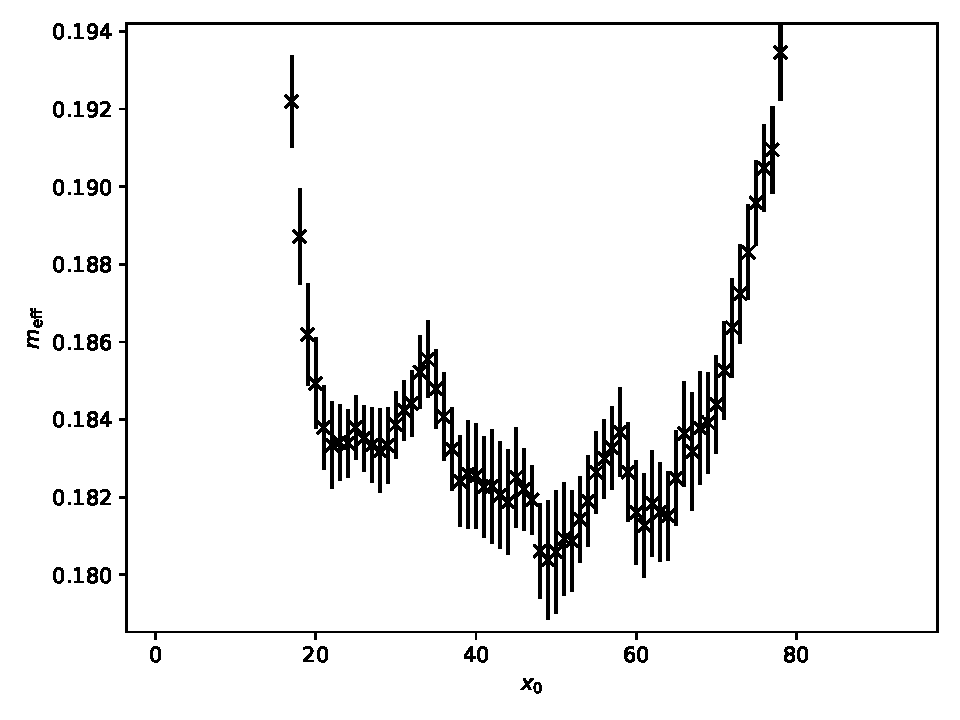
\includegraphics[width=\textwidth]{./cap3/figs/m_H101_pion_wil_plat.pdf}
    	\caption{}
    \end{subfigure}
    \begin{subfigure}{0.4\textwidth}
    	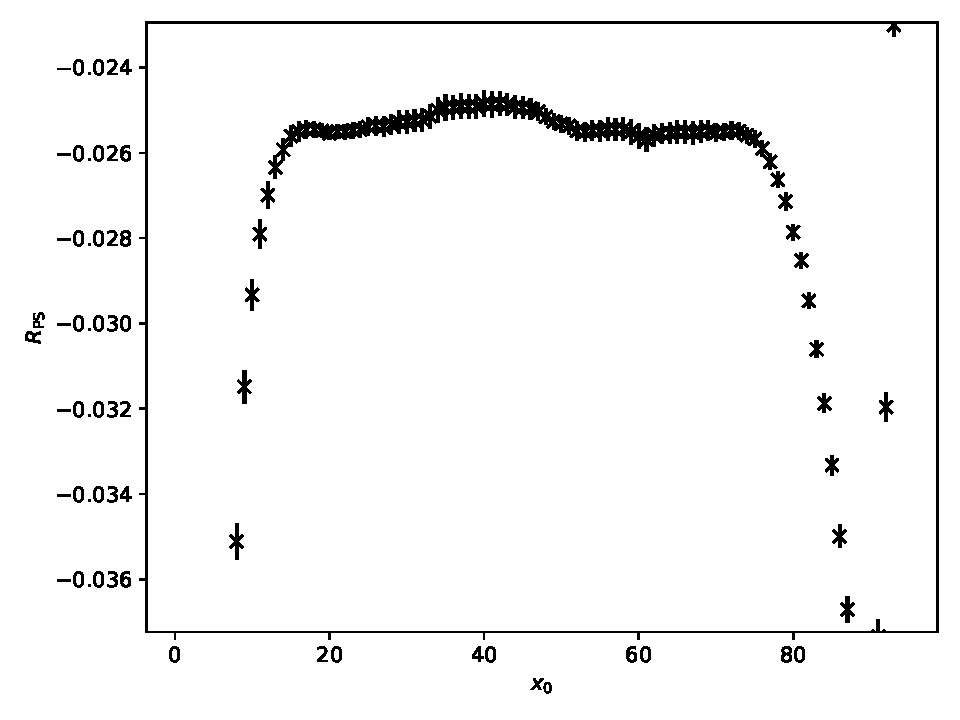
\includegraphics[width=\textwidth]{./cap3/figs/R_H101_pion_wil_plat.pdf}
    	\caption{}
    \end{subfigure}
    \begin{subfigure}{0.4\textwidth}
    	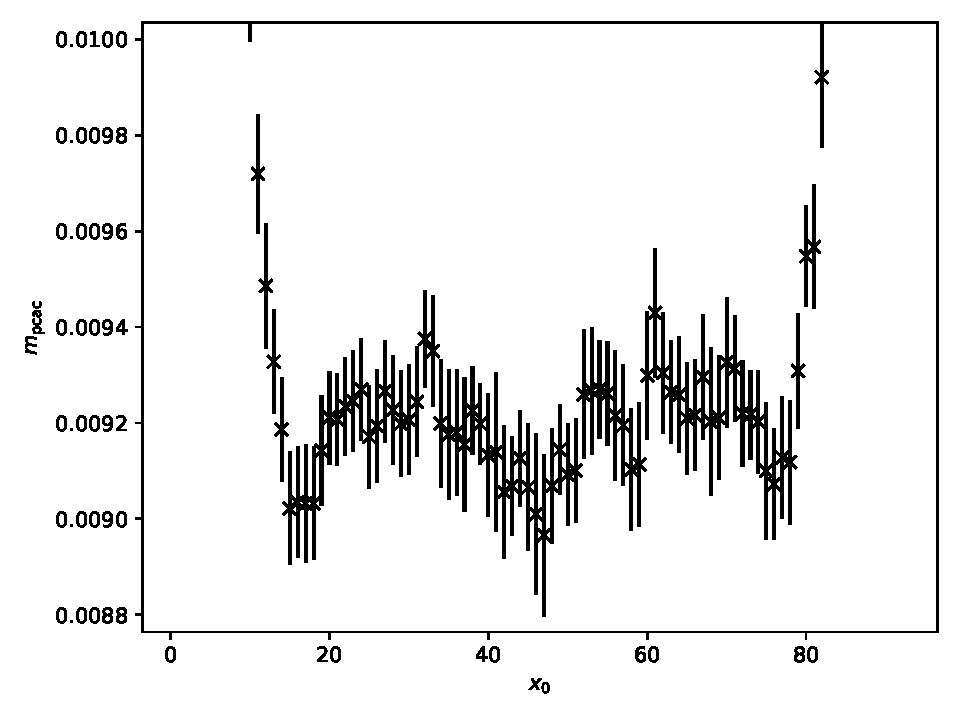
\includegraphics[width=\textwidth]{./cap3/figs/mpcac_H101_pion_wil_plat.pdf}
    	\caption{}
    \end{subfigure}
    \begin{subfigure}{0.4\textwidth}
    	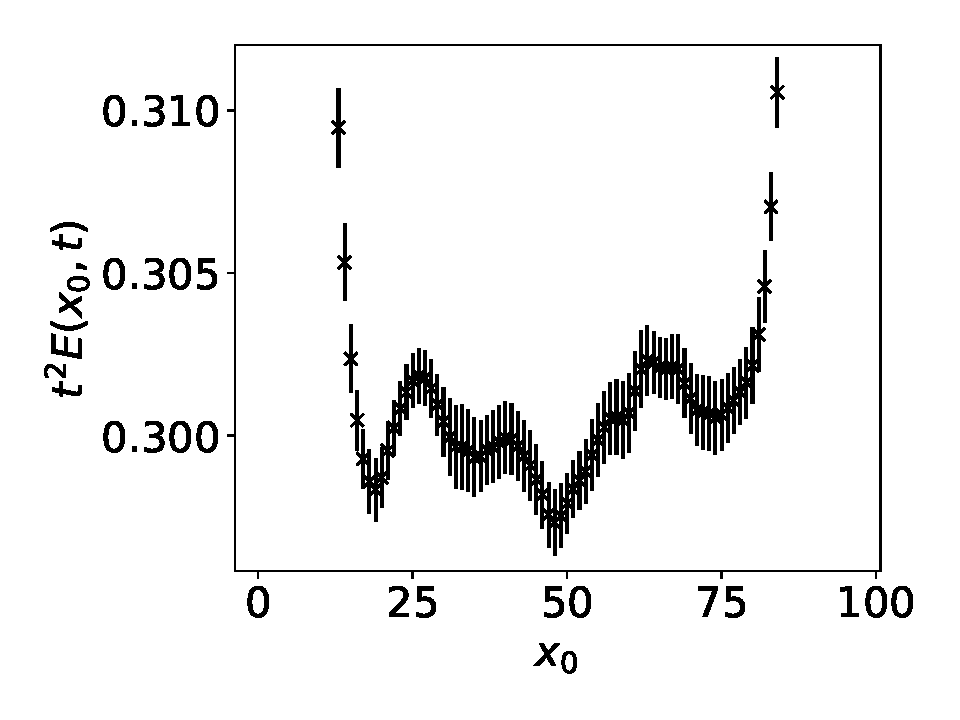
\includegraphics[width=\textwidth]{./cap3/figs/t2E_H101_plat.pdf}
    	\caption{}
    \end{subfigure}
    \begin{subfigure}{0.4\textwidth}
    	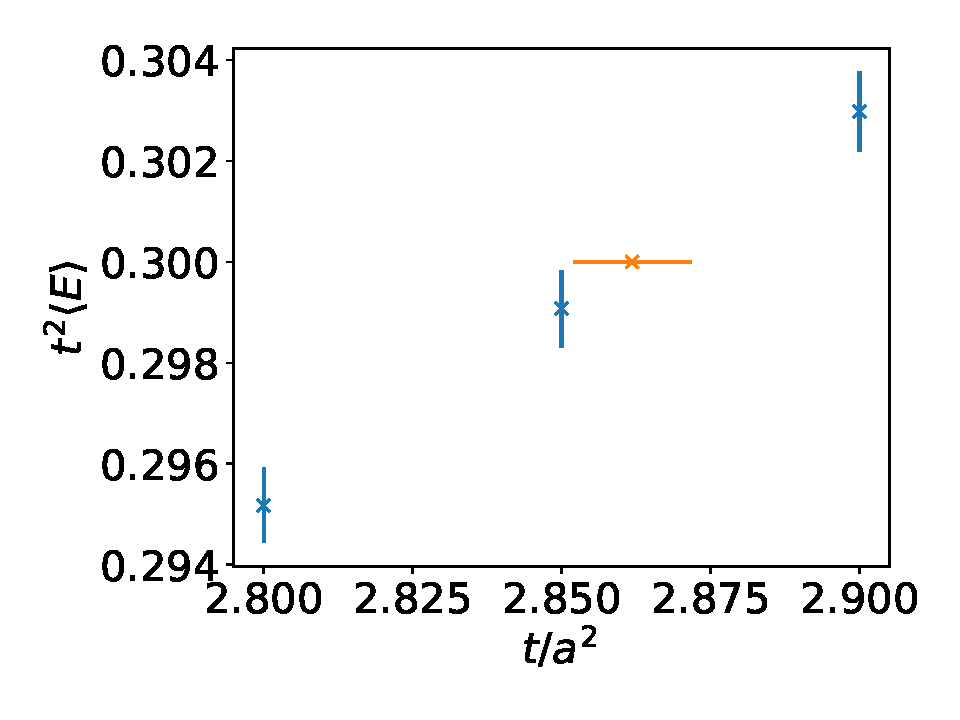
\includegraphics[width=\textwidth]{./cap3/figs/t0_H101.pdf}
    	\caption{}
    \end{subfigure}
    \caption{From (a) to (e) respectively: pion effective mass $m_{\textrm{eff}}$ in eq.~(\ref{ch_observables:eq:meff}), vacuum-to-pion axial matrix element $R_{\textrm{PS}}$ from eq.~(\ref{ch_observables:eq:R}), up-down PCAC quark mass in eq.~(\ref{ch_observables:eq:PCAC}), $t^2E(t)$ for a value of the flow time $t/a^2$ close to $t_0/a^2$ as defined in eq.~(\ref{ch_observables:eq:t0}), and values of $t^2E(t)$ for several flow times $t/a^2$ near $t_0/a^2$ (blue points) and the interpolated result for $t_0/a^2$ (orange point). All results are for ensemble H101 in the Wilson regularization.}
\end{figure}

\begin{figure}
\label{ch_observables:fig:model_av}
\centering
	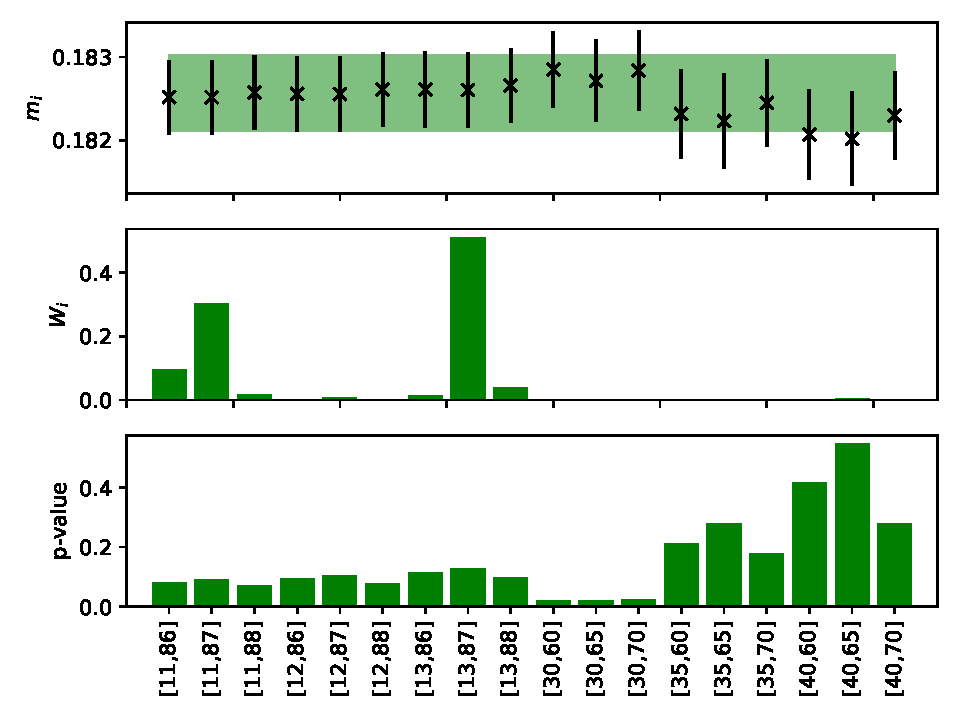
\includegraphics[width=.8\textwidth]{./cap3/figs/m_H101_pion_wil.pdf}
    \caption{Model variation for the extraction of the ground state signal in the pion effective mass of ensemble H101 in the Wilson regularization, shown in Fig.~\ref{ch_observables:fig:obs}. From top to bottom we show the ground state signal result from a fit to eq.~(\ref{ch_observables:eq:fit}) for each fit interval choice, the weight associated to each choice according to eq.~(\ref{ch_observables:eq:weight}), and the goodness of fit measured through the p-values defined in~\cite{}. We see that the highest weights are associated to a compromise between good fits (in terms of p-values) and fits with large number of points. The right-most models in the plot are heavily penalized even though they have the best p-values, since they cut a large number of points and models with not so severe cuts get also good p-values. The band in the top figure indicates the final weighted average result with the systematic uncertainty in eq.~(\ref{ch_observables:eq:syst}) included.}
\end{figure}


%%%%%%%%%%%%%%%%%%%%%%%%%%%%%%%%%%%%%%%%%%%%%%%%%%%%%%%%%%%
%%%%%%%%%%%%%%%%%%%%%%%%%%%%%%%%%%%%%%%%%%%%%%%%%%%%%%%%%%%
